\documentclass{article}
\usepackage{graphicx}
\usepackage{listings}
\usepackage{color}
\usepackage{amsmath}
\usepackage[utf8]{inputenc}

\title{Metodo di Eulero: un'implementazione\\
	Corso di LSMC, a.a. 2017-2018}
\author{Davide Gori\\
	550282}


\definecolor{backcolour}{rgb}{0.95,0.95,0.92}
\definecolor{gray}{rgb}{0.5,0.5,0.5}
\lstset{basicstyle=\ttfamily\small,
	columns=fullflexible,
	numbers=left,
	numberstyle=\tiny\ttfamily\color{gray},
	backgroundcolor=\color{backcolour},
	tabsize=4,
	language=Octave
}


\begin{document}
	\maketitle
	\section{Prima sperimentazione: implementazione metodo}
	Voglimamo scrivere un file di tipo function che implementi su una griglia uniforme il metodo di Eulero per la risoluzione del problema ai valori iniziali
	\begin{equation}
	\begin{cases}
	y'=f(x,y) \\
	y(0)=y_0
	\end{cases}
	\end{equation}
	\section{Lo script}
	Questo è lo script che realizza la sperimentazione:
	
	\lstinputlisting{eulero.m}
	
	\section{Seconda sperimentazione: un esempio}
	Vogliamo risolvere il seguente problema:
	\begin{equation}
	\begin{cases}
	y'=- \frac{2y+x^2 y^2}{x}, & x \in [1, 2] \\
	y(1)=1
	\end{cases}
	\end{equation}
	la cui soluzione esatta è $y(x)=\frac{1}{x^2 (1+\ln{x})}$
	\begin{itemize}
	\item La funzione {\tt fun} implementa l'equazione differenziale.
	\item Costruiamo il file script {\tt eser2\_1} che calcoli la soluzione approssimata ottenuta con il metodo di Eulero sulla griglia equispaziata di 11 punti. Disegnare la soluzione calcolata utilizzando una linea rossa e disegnare sullo stesso grafico la soluzione esatta in blu.
	\end{itemize}

	\section{Il codice}
	Questa è la funzione {\tt fun.m}:
	
	\lstinputlisting{fun.m}
	
	Questo è lo script {\tt LabSper\_1.m}:
	
	\lstinputlisting{LabSper_1.m}
	
	\section{Risultati}
	
	Riportiamo il grafico in output.
	
	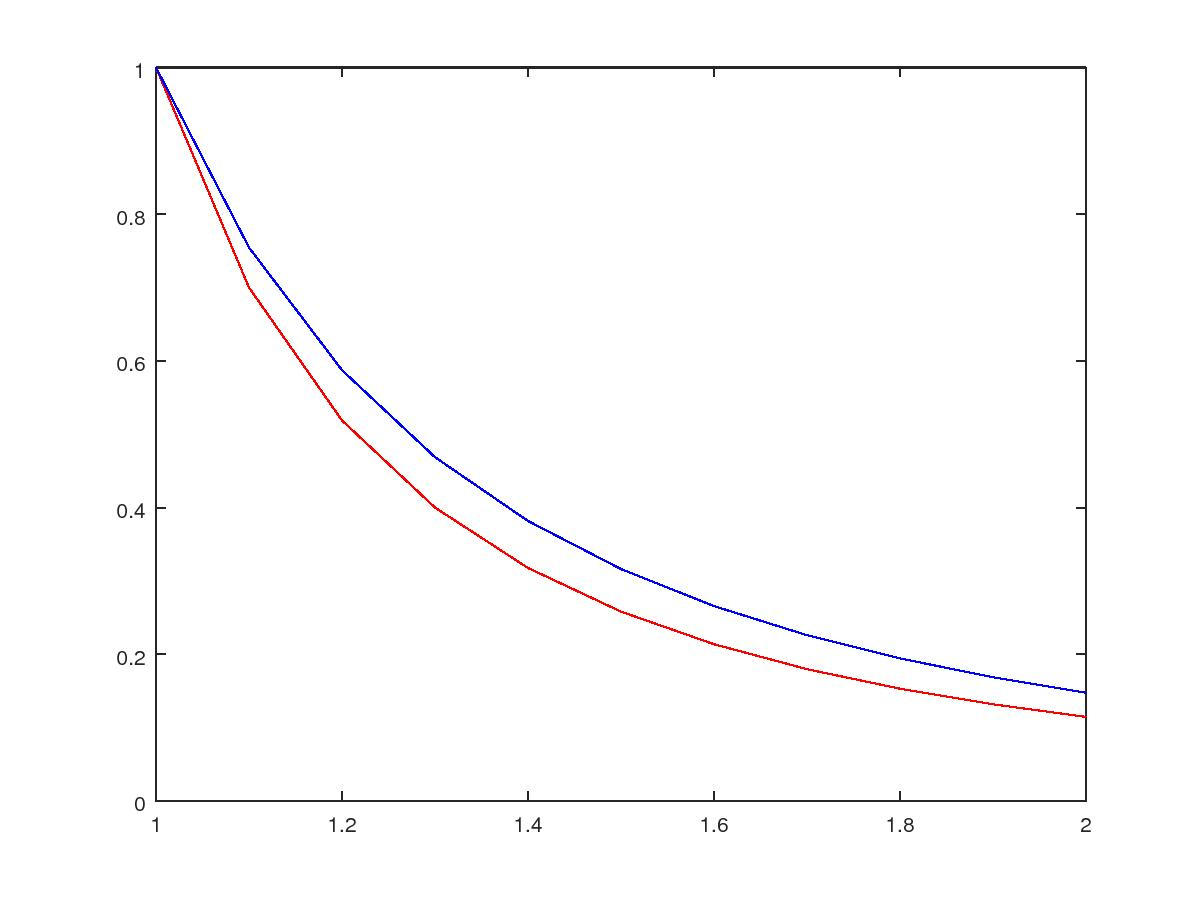
\includegraphics[width=\textwidth]{soluzioni.jpeg}
\end{document}